\chapter{Results} % Main chapter title

\label{chap:results} % For referencing the chapter elsewhere, use \ref{Chapter1} 

\section{Semantic Embeddings}
\subsection{Validation on English Data}
For \code{SIM} space, we used the English \code{WordNetEmbedding} trained on the first 15,000 frequent words and benchmark dataset vocabulary. The first 511 PCs are kept (Section \ref{subsec:semanticsimilaritymethod}), which is comparable to the best dimensionality (850) reported by the original work \parencite{saediWordNetEmbeddings2018} for a \code{WordNetEmbedding} trained with all semantic relations.

The intersection of \code{SIM} and the Common Crawl vocabulary used in \code{MIX} resulted to 8157 words. The linear regression model mapping \code{SIM} to \code{MIX} produced a \code{r2} score of 0.1662.

Figure \ref{fig:EngDecorVarRatio} shows the PCA-factored explained variances of the 4 resulting semantic space PCs. After PCA transformation, \emph{Similarity} spaces' explained variance are more concentrated on initial PCs while \association spaces are more homogeneously distributed. The concentration contrast suggests that \association spaces contain richer semantic information, consistent with the low \code{r2} found for the linear projection. In semantic ranking task evaluations (Table \ref{tab:engdecorrelationscores}), conformably to our hypotheses, the untouched \code{MIX} space is indeed a mixture of \similarity and \association information. \code{SIM}, which is constructed with specifically picked semantic relations from \code{WordNet}, is purely \similarity with statistically negligible \association scores. Though we have not completely purged \similarity information from \code{ASN} and \association from \code{SIG}, each resulting semantic space has significantly reduced the score in its irrelevant semantic axis. In addition, a clear dominance of \association semantic signal is present in \code{ASN} and \similarity in \code{SIG}. 


\begin{table}
    \centering
    \begin{ThreePartTable}
        
    \begin{tabularx}{\textwidth}{RRRRll}
        \multicolumn{6}{l}{\tabhead{English Semantic Space Semantic Ranking Task Results}} \\
    \toprule
    \tabhead{Semantic Space} & \tabhead{Vocabulary Size} & \tabhead{Dimension} & r & \tabhead{SimLex-999} & \tabhead{WS353-ASN} \\  
    \midrule
    \mr{2}{*}{\code{SIM}} & \mr{2}{*}{15K} & \mr{2}{*}{511} & Pearson & .5060 & \textbf{.0279}\tnote{1} \\  
    &  &  & Spearman & .4989 & \textbf{.0193}\tnote{2}   \\  
    \midrule
    \mr{2}{*}{\code{MIX}} & \mr{2}{*}{2.2M} & \mr{2}{*}{300} & Pearson & .3946 & .6091 \\  
    &  &  & Spearman & .3752 & .5709 \\  
    \midrule
    \mr{2}{*}{\code{ASN}} & \mr{4}{*}{8157} & \mr{4}{*}{300} & Pearson & .1953 & .5633 \\  
    &  &  & Spearman & .2133 & .5918 \\ 
    
    \cmidrule{1-1} \cmidrule{4-6}
    \mr{2}{*}{\code{SIG}} &  &  & Pearson & .4929 & .2091 \\  
    &  &  & Spearman & .4994 & .1678 \\  
    
    \cmidrule{2-6}
    \multicolumn{4}{r}{Out of Vocabulary} & .002 & .024 \\  
    \midrule \midrule
    \mr{2}{*}{Baseline\tnote{3}} & \mr{2}{*}{13k} & \mr{2}{*}{850} & Pearson & .50 & .32 \\  
        &  &  & Spearman & .52 & .33 \\  
    \bottomrule
    \end{tabularx}
    \begin{tablenotes}
        \footnotesize
        \item Scores marked in bold have a p-value larger than 0.05.
        \item[1] p-value=0.6626
        \item[2] p-value=0.7629
        \item[3] Baseline is reported by \textcite{saediWordNetEmbeddings2018}. The 13k words are selected cue words in psycholinguistic experiments. They show the best performance among all tested models.
    \end{tablenotes}
    \end{ThreePartTable}
    \caption[English Semantic Space Semantic Ranking Task Results]{With a different semantic relation selection, \code{SIM} achieves almost the same performance as the baseline in \similarity benchmark, while it cancels out the 
    \association score. \code{MIX} space performs well in both task-sets, with a slight preference for \association, consistent with \parencite{lapesaContrastingSyntagmaticParadigmatic2014}'s conclusion. \code{ASN} has comparable scores in \association with \code{MIX}, but still have a non-zero score in \similarity. The projected \code{SIG} space compared with \code{SIM} has similar scores in \similarity and a much lower score in \association.\label{tab:engdecorrelationscores}}
    \end{table}

\subsection{Application on French data}

Provided with the methodological success of English data, we applied the same algorithm against French data.

For \code{SIM} space, we used the French \code{WOLFEmbedding} with POS tag trained on all the available vocabulary. The first 634 PCs are kept.

After rule-based and manual matching, the intersection of \code{SIM} space and the \code{MIX} space vocabulary resulted to 24519 distinct lemma with POS tags.

The linear regression model mapping \code{SIM} to \code{MIX} produced a \code{r2} score of 0.0776, which is lower than the English score, indicating a smaller informational overlap between the two embedding models.

Figure \ref{fig:FreDecorVarRatio} shows a similar PCA explained variance distribution to English, but the French \code{SIG} seems have a denser concentration of EVR in first PCs than \code{SIM}, which is not the case with English spaces. We tested the resulting semantic spaces using the same tasks against our indicative gold-standard data  (Table \ref{tab:fredecorrelationscores}), without sound evidence supporting the validity of the results. The unmodified \code{MIX} space has a much lower score in \similarity and \association compared to the English \code{MIX}, possibly due to the poor quality of benchmarks, setting a weak baseline for embedding space comparison. 
Again, \code{SIM} achieves high scores in \emph{similarity}, and negligible scores in \emph{association}. \code{SIG} seems to contain lesser (or purer) information than \code{SIM} by PC examination, which is convergent with the the comparable \similarity scores as \code{SIM} and the more remarked purity against \association tests. However, the Pearson's and Spearman's \code{r} reporting from the tests gave contradicting conclusions on \code{ASN}, which leads us to further examinations of \code{ASN}'s linguistic property. It is worth noting that the \association scores of \code{ASN} are nevertheless higher than \similarity scores. 

\begin{table}
    \centering
    \begin{ThreePartTable}
    
    \begin{tabularx}{\textwidth}{RRRR *{2}{A{2.3cm}}}
        \multicolumn{6}{l}{\tabhead{French Semantic Space Semantic Ranking Task Results}} \\
    \toprule
    \tabhead{Semantic Space} & \tabhead{Vocabulary Size} & \tabhead{Dimension} & r & \tabhead{\emph{Similarity} SimLex-999} & \tabhead{\emph{Association} WS353-ASN} \\  
    \midrule
    
    \mr{5}{*}{\code{SIM}} & \mr{4}{*}{56665} & \mr{4}{*}{634} & Pearson & .3291 & \textbf{.1039} \\  
    &  &  & p-value & 0 & .1061 \\  
    \cmidrule{4-6}
    &  &  & Spearman & .2812 & \textbf{.0511} \\  
    &  &  & p-value & 0 & .4273 \\  
    \cmidrule{2-6}

    \multicolumn{4}{r}{Out of Vocabulary} & .048 & .04 \\  
   \midrule

   \mr{4}{*}{\code{MIX}} & \mr{14}{*}{24519} & \mr{14}{*}{200} & Pearson & .0940 & .1520 \\  
   &  &  & p-value & .0047 & .0197 \\  
   \cmidrule{4-6}

    &  &  & Spearman & .1449 & .2078 \\ 
    &  &  & p-value & 0 & .0014 \\  

    \cmidrule{1-1} \cmidrule{4-6}

   \mr{4}{*}{\code{ASN}} &  &  & Pearson & \textbf{.0629} & \textbf{.1116} \\  
   &  &  & p-value & .0590 & .0879 \\  
   \cmidrule{4-6} 
    &  &  & Spearman & .0771 & .1566 \\  
    &  &  & p-value & .0206 & .0162 \\  

\cmidrule{1-1} \cmidrule{4-6}

   \mr{4}{*}{\code{SIG}} &  &  & Pearson & .2541 & \textbf{-.0044} \\  
   &  &  & p-value & 0 & .9458 \\  
   \cmidrule{4-6}

    &  &  & Spearman & .3121 & \textbf{-.0078} \\  
   &  &  & p-value & 0 & .9050 \\  

    \cmidrule{2-6}

    \multicolumn{4}{r}{Out of Vocabulary} & .0797 & .0711 \\  

    \bottomrule
    \end{tabularx}
    \begin{tablenotes}
        \footnotesize
        \item[] The tested null hypothesis is a non-existent linear correlation between the model predicted scores and the gold-standard. Scores marked in bold have a p-value larger than 0.05.
    \end{tablenotes}
    \end{ThreePartTable}
    
    \caption[French Semantic Space Semantic Ranking Task Results]{Possibly due to the poor quality of French benchmark datasets, baseline scores with \code{MIX} is much lower than the English counterpart. \code{SIM} has high performance in \similarity and negligible \association scores. The relatively poor de-correlation between \code{SIM} and \code{MIX} resulted a debatable \code{ASN}. Viewed by Pearson's \code{r} it seems to contain none of \similarity and \association information, judged by Spearman's \code{r}, both axes' information are present in the space. All p-values reported for \code{ASN} are close to the significance threshold. Still, \code{ASN} holds higher scores in \association than \similarity. \code{SIG} however, cancels out completely \association information even compared with \code{SIM} while retained \similarity signals.}
    % the results puts the validity of \code{ASN} space into question:  
    \label{tab:fredecorrelationscores}
    \end{table}

To clarify on the nature of \code{ASN} due to the found debatable results, we visualized the French \code{ASN} along with other semantic spaces using an embedding projector\footnote{Published as a TensorFlow component, available at \url{https://projector.tensorflow.org/}. The entries in the embedding space is presented by a sphere positioned in a 3D space, of which the coordinates are by default calculated with the first 3 PCs.} to visualize several exemplar lexicon units and its vectorial neighbors. The examples in Section \ref{appsubsec:projectorvisu}) seems to show that French \code{ASN} has a predominant \association preference.


\section{Computational Analysis of Ridge Regression}

\subsection{Regressor Generation}

\subsubsection{Vocabulary Coverage}
Around 6\% of the content word occurrences and 7\% of the lexicon are not available in our obtained spaces (Table \ref{tab:lppcoverage} and \ref{apptab:lppcoverage}), potentially harming the quality of semantic regressors. 

\begin{table}
    \centering
    \begin{ThreePartTable}  
    \begin{tabularx}{\textwidth}{L *{10}{R}}
    \multicolumn{11}{l}{\tabhead{The Little Prince Vocabulary Coverage}} \\
    \toprule
    &  & \multicolumn{9}{l}{\tabhead{\# Instances in fMRI Recording Session}} \\
    \toprule
    &  & \tabhead{R1} & \tabhead{R2} & \tabhead{R3}& \tabhead{R4}& \tabhead{R5}& \tabhead{R6}& \tabhead{R7}& \tabhead{R8}& \tabhead{R9}\\
    \toprule

    \mr{2}{*}{Story} & \textbf{T} & 725 & 812 & 860 & 762 & 732 & 902 & 819 & 712 & 802 \\
    & \textbf{V} & 348 & 360 & 411 & 329 & 292 & 367 & 302 & 328 & 343 \\
    \midrule
    \mr{4}{*}{\parbox{0.8cm}{\code{SIM} 56665}} & TM & 36 & 30 & 32 & 27 & 30 & 33 & 24 & 30 & 27 \\
    & \% & 4.97 & 3.69 & 3.72 & 3.54 & 4.10 & 3.66 & 2.93 & 4.21 & 3.37 \\
     & VM & 26 & 16 & 22 & 20 & 16 & 19 & 16 & 19 & 16 \\
     & \% & 7.47 & 4.44 & 5.35 & 6.08 & 5.48 & 5.18 & 5.30 & 5.79 & 4.66 \\
    \midrule
    \mr{4}{*}{\parbox{0.8cm}{\code{ASN} /\code{MIX} /\code{SIG} 24519}} & TM & 48 & 47 & 38 & 37 & 48 & 60 & 35  & 37 & 41 \\
    & \% & 6.62 & 5.79 & 4.42 & 4.86 & 6.56 & 6.65 & 4.27 & 5.20 & 5.11 \\
     & VM & 30 & 26 & 26 & 25 & 26 & 32 & 20 & 22 & 25 \\
     & \% & 8.62 & 7.22 & 6.33 & 7.60 & 8.90 & 8.72 & 6.62 & 6.71 & 7.29 \\
    \bottomrule
    \end{tabularx}
    \end{ThreePartTable}
    \caption[The Little Prince Vocabulary Coverage in Semantic Spaces]{Only content words are taken into consideration. \textbf{T}: Token, \textbf{V}: Distinct Lexicon Unit, M: Miss\label{tab:lppcoverage}}
    \end{table}

\subsubsection{Corpus-Targeted Semantic Feature Selection}

After having generated regressors with word onset timestamps and semantic representation vectors, the average variance cross 9 groups of 634 resulting regressors (Section \ref{subsec:semanticsimilaritymethod}) are computed and visualized in Figure \ref{fig:freSIMRegVar}. Since we target less than 200 regressors and the dependency of regressors (due to orthonormalization) is to conserve, we visually selected the threshold of \(10^{-5}\), which resulted 100 informative regressors for \code{SIM} space\footnote{The selected dimensions are 1 -- 85, 87 -- 94, 96, 97, 99, 100, 103, 117, 131.}.

\begin{figure}
    \centering
    \makebox[\linewidth]{
    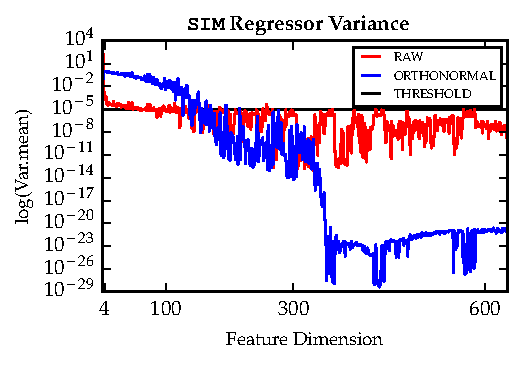
\includegraphics[scale=1]{Figures/SimDimensionSelectionRegLPP.pdf}
    }
    \caption[French \code{SIM} Regressor Variances]{The average of 9 fMRI run semantic regressor variances. There are 3 non-embedding regressors, and 634 \code{SIM}-based regressors. \code{RAW} stands for regressor values directly after hemodynamic convolution, \code{ORTHONORMAL} stands for de-linearized regressors after Gram-Schmidt process. \code{THRESHOLD} for regressor selection is fixed at \(10^{-5}\). The \code{RAW} regressors' variance declines dramatically after first few \code{SIM} regressors (dim > 3), and stays relatively stable for later dimensions. This observed trend corresponds globally well to the eigenvalue evolution of \code{SIM} space (Figure \ref{fig:FreDecorVarRatio}). \code{RAW} curve indeed shows a few dimension's smaller variance compared to Figure \ref{fig:SimDimensionSeletionVarRatio}. \code{ORTHONORMAL} regressors's variance declines more slowly, and has a noised plateau around dimension 100 -- 300. Posterior positioned regressors suffer more significantly in variance (smaller than \(10^{-23}\), approaching the computation precision limit of Python \code{float}s) and retained almost no information for the second half PCs. The regressors are orthonormalized, so removing an anteriorly positioned regressor breaks the information completeness of posterior ones. The threshold is cut around the upper bound of the \code{ORTHONORMAL} variance plateau noise, so a continuous regressor set could be included in the final design matrix without surpassing the dimensionality limit (of 200 which is the dimensionality of the used DepGlove embedding).} 
    \label{fig:freSIMRegVar}
\end{figure}


\subsection{Choice of \(\alpha\) and Effective Feature Dimensionality}

% Our pilot regression experiments partially replicated the original experience \parencite{verdierEncodageActiviteNeuronale2018} with French data on the voxel-model performance spatial-patterns and performance improvement only if we fix the regularization parameter for non-semantic and semantic models (\code{MIX}). The results indicate that fixing one parameter for all models cannot fully exploit the power of the supplied regressors. The fixed \(\alpha\) preferentially improves the regression performance for certain models. 

For each of four semantic models, we generated design matrices for each fMRI session with 103 or 203 features (including 3 non semantic embedding features). 

Figure \ref{fig:MIX_HeatmapAlphaDimS1R0} plots the best hyper-parameter distribution based on the average \code{r2} score of subject 1, \code{MIX} model. This example, together with session-wise, and other subject-wise visualization of all semantic models\footnote{The visualizations are available online at \url{http://bit.ly/micipsa_heatmaps}.} suggests that our research space for \(\alpha\) and feature-dimension parameters are complete: the distribution of voxel-configurations are bounded by our search space. Section \ref{appsubsec:alphadim} details the analysis. The interaction between \(\alpha\) values and voxel regression performances supports our decision of testing voxel-specific Ridge configuration.

\begin{figure}
\centering
        \makebox[.5\linewidth]{
            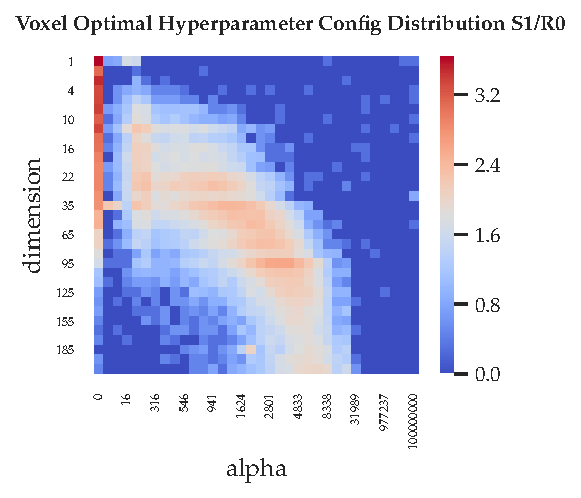
\includegraphics[scale=.8]{Figures/MIX_HeatmapAlphaDimS1R0.pdf}
            }
            \caption[Subject Best Hyper-parameter Configuration Voxel-Count Heat-map]{After averaging \code{MIX} best \code{r2}s across 9 runs of one same subject, best hyper-parameter configuration appears to be regularly distributed below the diagonal of the visualized search space. A large proportion of voxels are best modeled with no Ridge regularization (especially for voxels using <4 features). Voxel-models requiring for higher-dimensional features are associated with larger \(\alpha\) values. \(\alpha > 10^{4.5} (31989)\) rarely achieves best predictive performances, suggesting that the \(\alpha\) search space is complete for the subject.} 
            \label{fig:MIX_HeatmapAlphaDimS1R0}
\end{figure}

\section{Cognitive Analysis of fMRI Encoding}

Only the group-level results and analyses are presented. Subject-wise data are also made available via the links provided in each section.

\subsection{Non Semantic-Embedding Models}

%Contrast Map
\begin{figure}
    \centering
    \makebox[\linewidth]{
    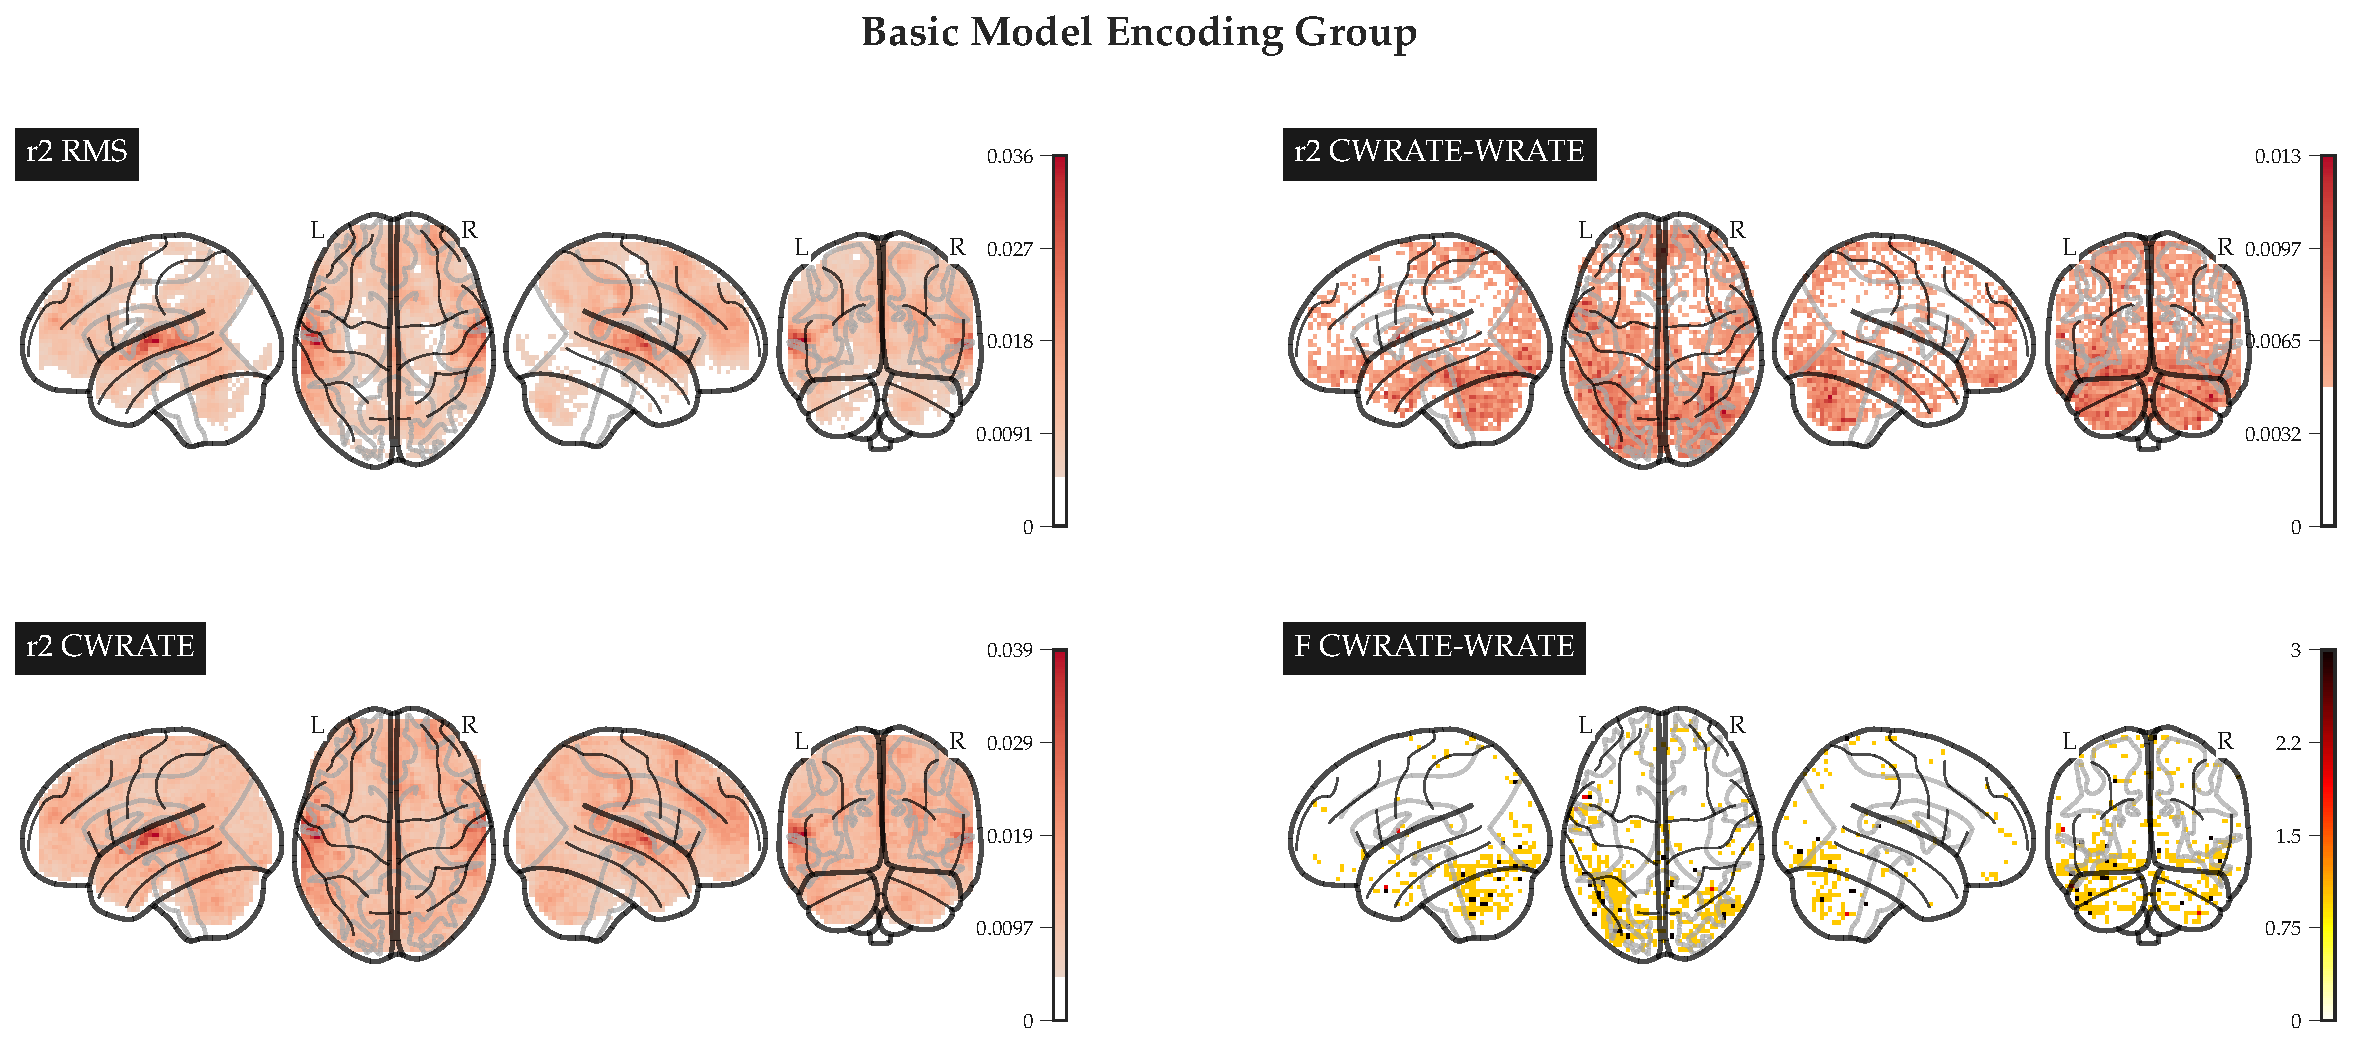
\includegraphics[width=.8\paperwidth]{Figures/BASE_ContrastMapG.pdf}
    }
    \caption[Encoding with \code{BASE} Features, Group]{\textbf{Left panels} are plots of voxel-wise \code{r2} scores for three \emph{classes} of non semantic-embedding regressors. With \code{RMS}, \code{WRATE} and \code{CWRATE}, consistent model performances are found for bilateral primary auditive cortices, with a slight preference for left hemisphere (Table \ref{tab:rmsCluters}). \textbf{Right upper panel} is the \code{r2} improvement map of \code{CWRATE} over \code{WRATE}. \code{CWRATE} improvements are mainly located in bilateral TP, ITG, frontopolar PFC and cerebellum near Fusiform gyrus (Table \ref{tab:cwrateImprovementClusters}). \textbf{Right lower panel} is the F-test contrasting \code{RMS+WRATE+CWRATE} and \code{RMS+WRATE}. 3 levels of significance \code{1, 2, 3} are shown on the whole-brain map, corresponding respectively to p-values of uncorrected 0.05, 0.001 and voxel-wise corrected 0.05. Isolated voxels are reported in bilateral mid occipital, lingual BA17/18, right precuneus and cerebellum (Table \ref{tab:Ftest}).} 
    \label{fig:BASE_ContrastMapG}
\end{figure}

%r2 histogram
\begin{figure}
    \centering
    \makebox[\linewidth]{
    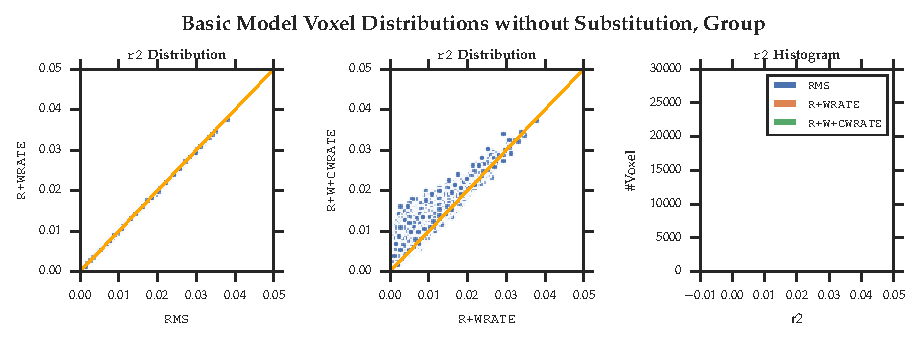
\includegraphics[width=\textwidth]{Figures/BASE_r2_Distribution.pdf}
    }
    \caption[Histogram of \code{r2} with \code{BASE} Features]{The voxel scores are averaged over all cross-validations of all subjects. The plotted scores are not substituted even if the model overfits. \textbf{Left panel} shows that the addition of \code{WRATE} does not improve any voxel's model performance. \textbf{Mid panel} suggests that \code{CWRATE} slightly overfits a small portion of voxels, the improvement for most voxels are minute. \textbf{Right panel}: However for originally randomly-modeled voxels (x-axis from 0--0.01), \code{CWRATE} does bring significant improvements. The group average suggests the benefit of adding \code{CWRATE} for a large proportion of voxels, which is not the case for subject results. Subject-wise scores are significantly higher (up to 0.2) and the score variability and overfitting are more remarkable.} 
    \label{fig:histo_base_best_nonsub_G}
\end{figure}

%clusters
% \begin{figure}
%     \centering
%     \makebox[\linewidth]{
%     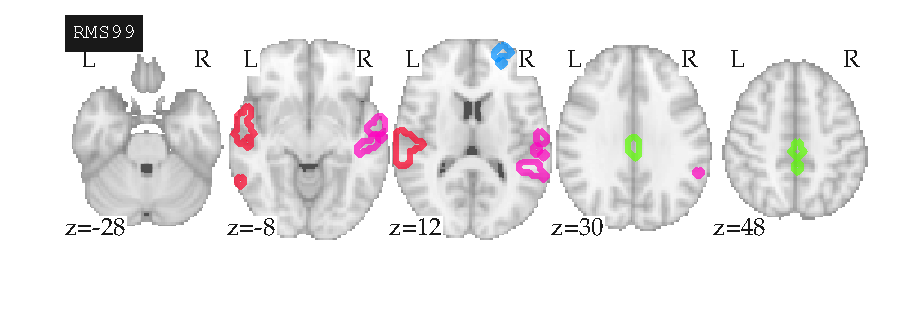
\includegraphics[width=.5\paperwidth]{Figures/RMS99_ClusterG.pdf}
%     }
%     \caption[\code{RMS} Top 1\% Voxel Clusters, Group]{[TODO remove?] With \code{RMS}, the best 1\% modeled voxels (with \code{r2}>0.0240) form 4 clusters containing more than 47 voxels. The two most large clusters are located in bilateral primary auditory cortices (BA41), a slight left-hemisphere preference is found (Left best \code{r2} 0.0362, cluster size 410 voxels, versus right best \code{r2} 0.0328 cluster size 337). Other two smaller clusters are located in right mid cingulum and right mid frontal cortex. The four-cluster structure is stable across \code{RMS}, \code{WRATE}, \code{CWRATE} and \code{SIM} \emph{feature classes}.} 
%     \label{fig:RMS99_ClusterG}
% \end{figure}

For acoustic features, \code{RMS} preferentially models voxels in bilateral Brodmann Area (BA) 41 (posterior superior temporal gyrus, pSTG), with a slight left lateralization (Figure \ref{fig:BASE_ContrastMapG} upper-left, Table \ref{tab:rmsCluters}). BA41 is part of the primary auditory (PA) cortex, and the left lateralization for speech is consistent with our finding~\parencite{tervaniemiLateralizationAuditorycortexFunctions2003}.

The addition of \code{WRATE} does not bring any impact (Figure \ref{fig:histo_base_best_nonsub_G} left panel), possibly due to the high co-linearity with \code{RMS} by definition, thus the orthonormalized feature contains only uninformative noises despite a relatively important variance (0.96 after orthonormalization). 

In contrast, \code{CWRATE} has only 0.10 variance (in comparison with \code{WRATE}), however, most voxels received better performance when the feature is added (Figure \ref{fig:histo_base_best_nonsub_G} middle panel). These improvements does not change the global voxel ranking. Still being two major voxel-clusters among the best modeled voxels, the bilateral PA clusters show a more pronounced lateralization towards the left hemisphere (Table \ref{tab:rmsCluters}). It suggests that additionally to speech primary auditory processing, left pSTG BA41 is also more implicated in the semantic aspect. 

The major improvement of \code{CWRATE} is remarked in left middle and inferior temporal pole (TP) BA38, bilateral posteroinferior temporal gyrus (ITG, including fusiform gyrus FG) BA19/37, frontopolar prefrontal cortex (fpPFC, near rectus gyrus) and posterior cerebellum (Table \ref{tab:cwrateImprovementClusters}, W=136, \(\Delta\)\code{r2}>0.0067, p-value<\(10^{-3.66}\) uncorrected). Isolated voxels are also reported in bilateral mid occipital, lingual BA17/18, right precuneus and cerebellum (Table \ref{tab:Ftest}, p-value<0.05 voxel-wise multi-comparison corrected). The left mid\slash inferior TP is associated to social concepts, the fusiform centroid is located near visual word form area, the precuneus cluster sits near anterior sensorimotor subdivisions. Subject-wise results are available online.\footnote{Whole-brain maps: \url{http://bit.ly/micipsa_base_wholebrain}. Histograms: \url{http://bit.ly/micipsa_regression_histogram}.}.

\subsection{\emph{Similarity} Nested Model}

\begin{figure}
    \centering
    \makebox[\linewidth]{
    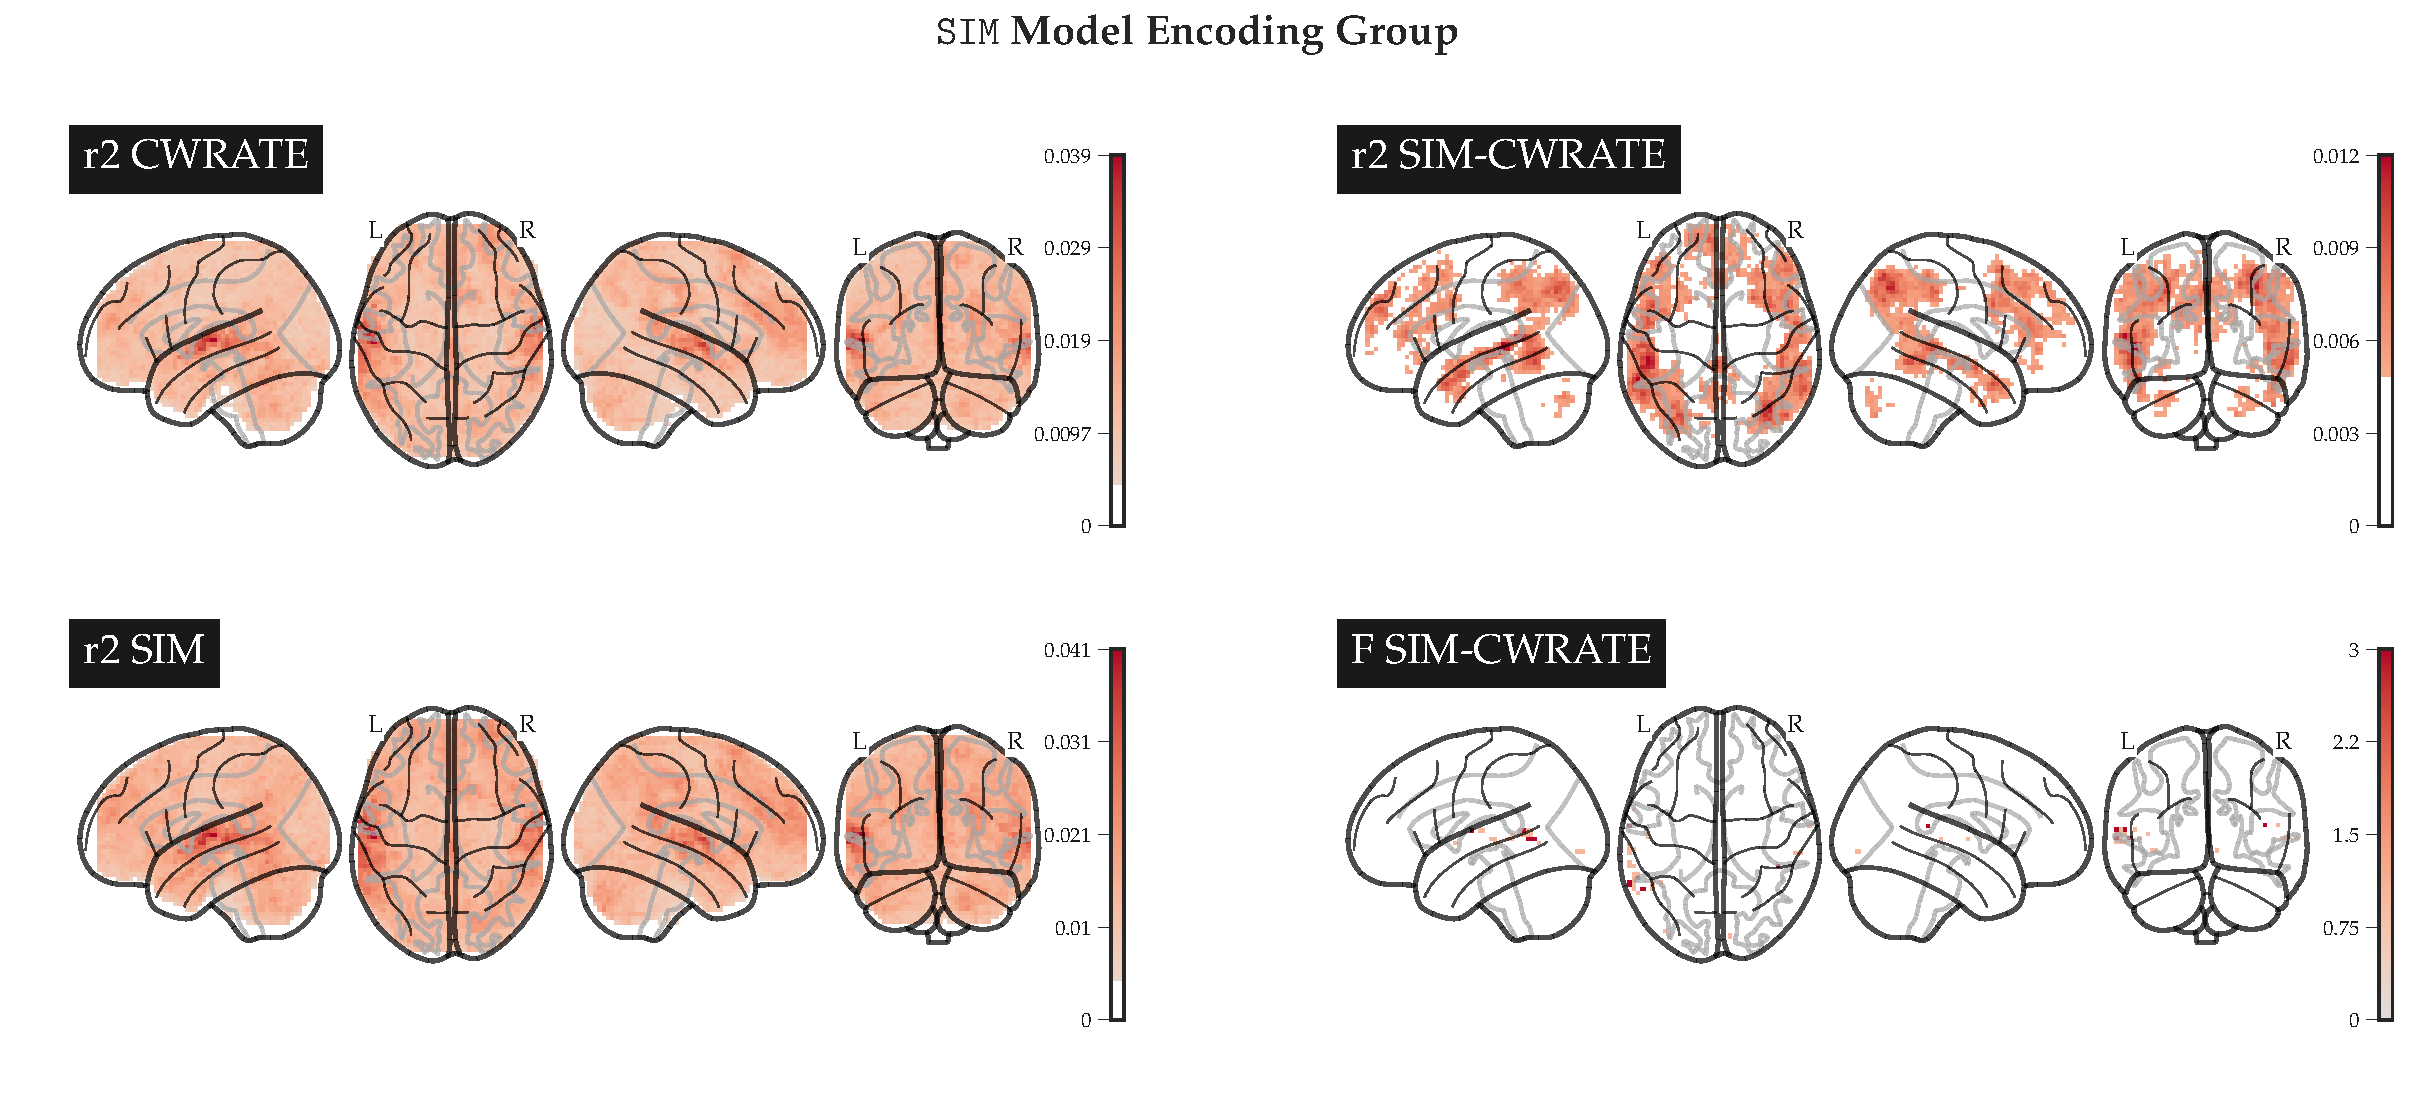
\includegraphics[width=.8\paperwidth]{Figures/SIM_ContrastMapG.pdf}
    }
    \caption[Encoding with \code{SIM} Features, Group]{\textbf{Left panels}: The global activation pattern is unchanged with the feature addition. Best modeled zones are bilateral primary auditory cortices. \textbf{Right upper panel}  shows that \code{SIM} better models bilateral middle TG (MTG), superior parietal lobule (SPL), angular gyrus (AG) (part of Wernicke's area), supramarginal gyrus (SMG) and prefrontal areas (Table \ref{tab:simImprovementClusters}). F-test in \textbf{right lower panel} reports a few significant voxels in left pMTG BA21, 39, right pSTG BA22 and left Heschl BA4 (Table \ref{tab:Ftest}).} 
    \label{fig:SIM_ContrastMapG}
\end{figure}

\begin{figure}
    \centering
    \makebox[\linewidth]{
    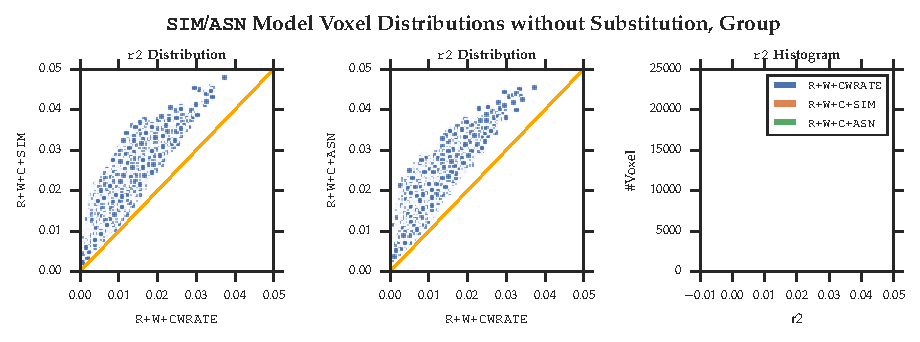
\includegraphics[width=.8\paperwidth]{Figures/SIM_ASN_Distribution.pdf}
    }
    \caption[Histogram of \code{r2} with \code{SIM/ASN} Features]{The group average of semantic embedding models make both important contributions for voxel-modeling (\textbf{left} and \textbf{mid} panels). \textbf{Right} panel shows that \code{ASN} model scores are distributed around a higher average (0.014) than \code{SIM} (0.01). Again, the subject-wise distributions show very different patterns than the group average: much higher \code{r2} and plenty of overfitted voxels.} 
    \label{fig:SIM_ASN_Distribution}
\end{figure}


We added \code{SIM} features upon non semantic-embedding models to trying to locate neural structures participating in semantic \similarity processing. While the whole-brain activation pattern stays globally unchanged (Figure \ref{fig:SIM_ContrastMapG} left, Table \ref{tab:rmsCluters}). \code{SIM} enlarges the performance superiority of left PA over right, suggesting a left preference for textual semantic \similarity processing. The \code{r2} distribution analysis (Figure \ref{fig:SIM_ASN_Distribution} left) shows that in group-average \code{SIM} is informative for most of the voxel-models and none of voxels is overfitted by this addition. The most improved voxel clusters are located in bilateral MTG (left improvement is more extensive, significant and medial), left superior parietal lobule and right angular gyrus (AG) (Table \ref{tab:simImprovementClusters}, W=210, \(\Delta\)\code{r2}>0.0079, p<\(10^{-4.35}\) uncorrected). F-test also reports left pMTG BA21/39, right pSTG BA22 (Table \ref{tab:Ftest}, p<0.05 voxel-wise multi-comparison corrected). The right pSTG locus is located within Wernicke's area. 

Bilateral pMTGs are connected with word-meaning access across modalities and categories of concept~\parencite{visserBothMiddleTemporal2012} and was also proposed as a semantic hub~\parencite{turkenNeuralArchitectureLanguage2011}. AG is argued to be associated with spatial attention, and controversially with metaphor understanding. SPL is linked to language association activations and visuo-motor coordination. \code{SIM} seems also to improve \association structures. Subject-wise results are available online\footnote{Whole-brain maps: \url{http://bit.ly/micipsa_sim_wholebrain}. Histograms: \url{http://bit.ly/micipsa_regression_histogram}.}.

\subsubsection{\emph{Similarity} Nested Model with \code{SIG}}

\begin{figure}
    \centering
    \makebox[\linewidth]{
        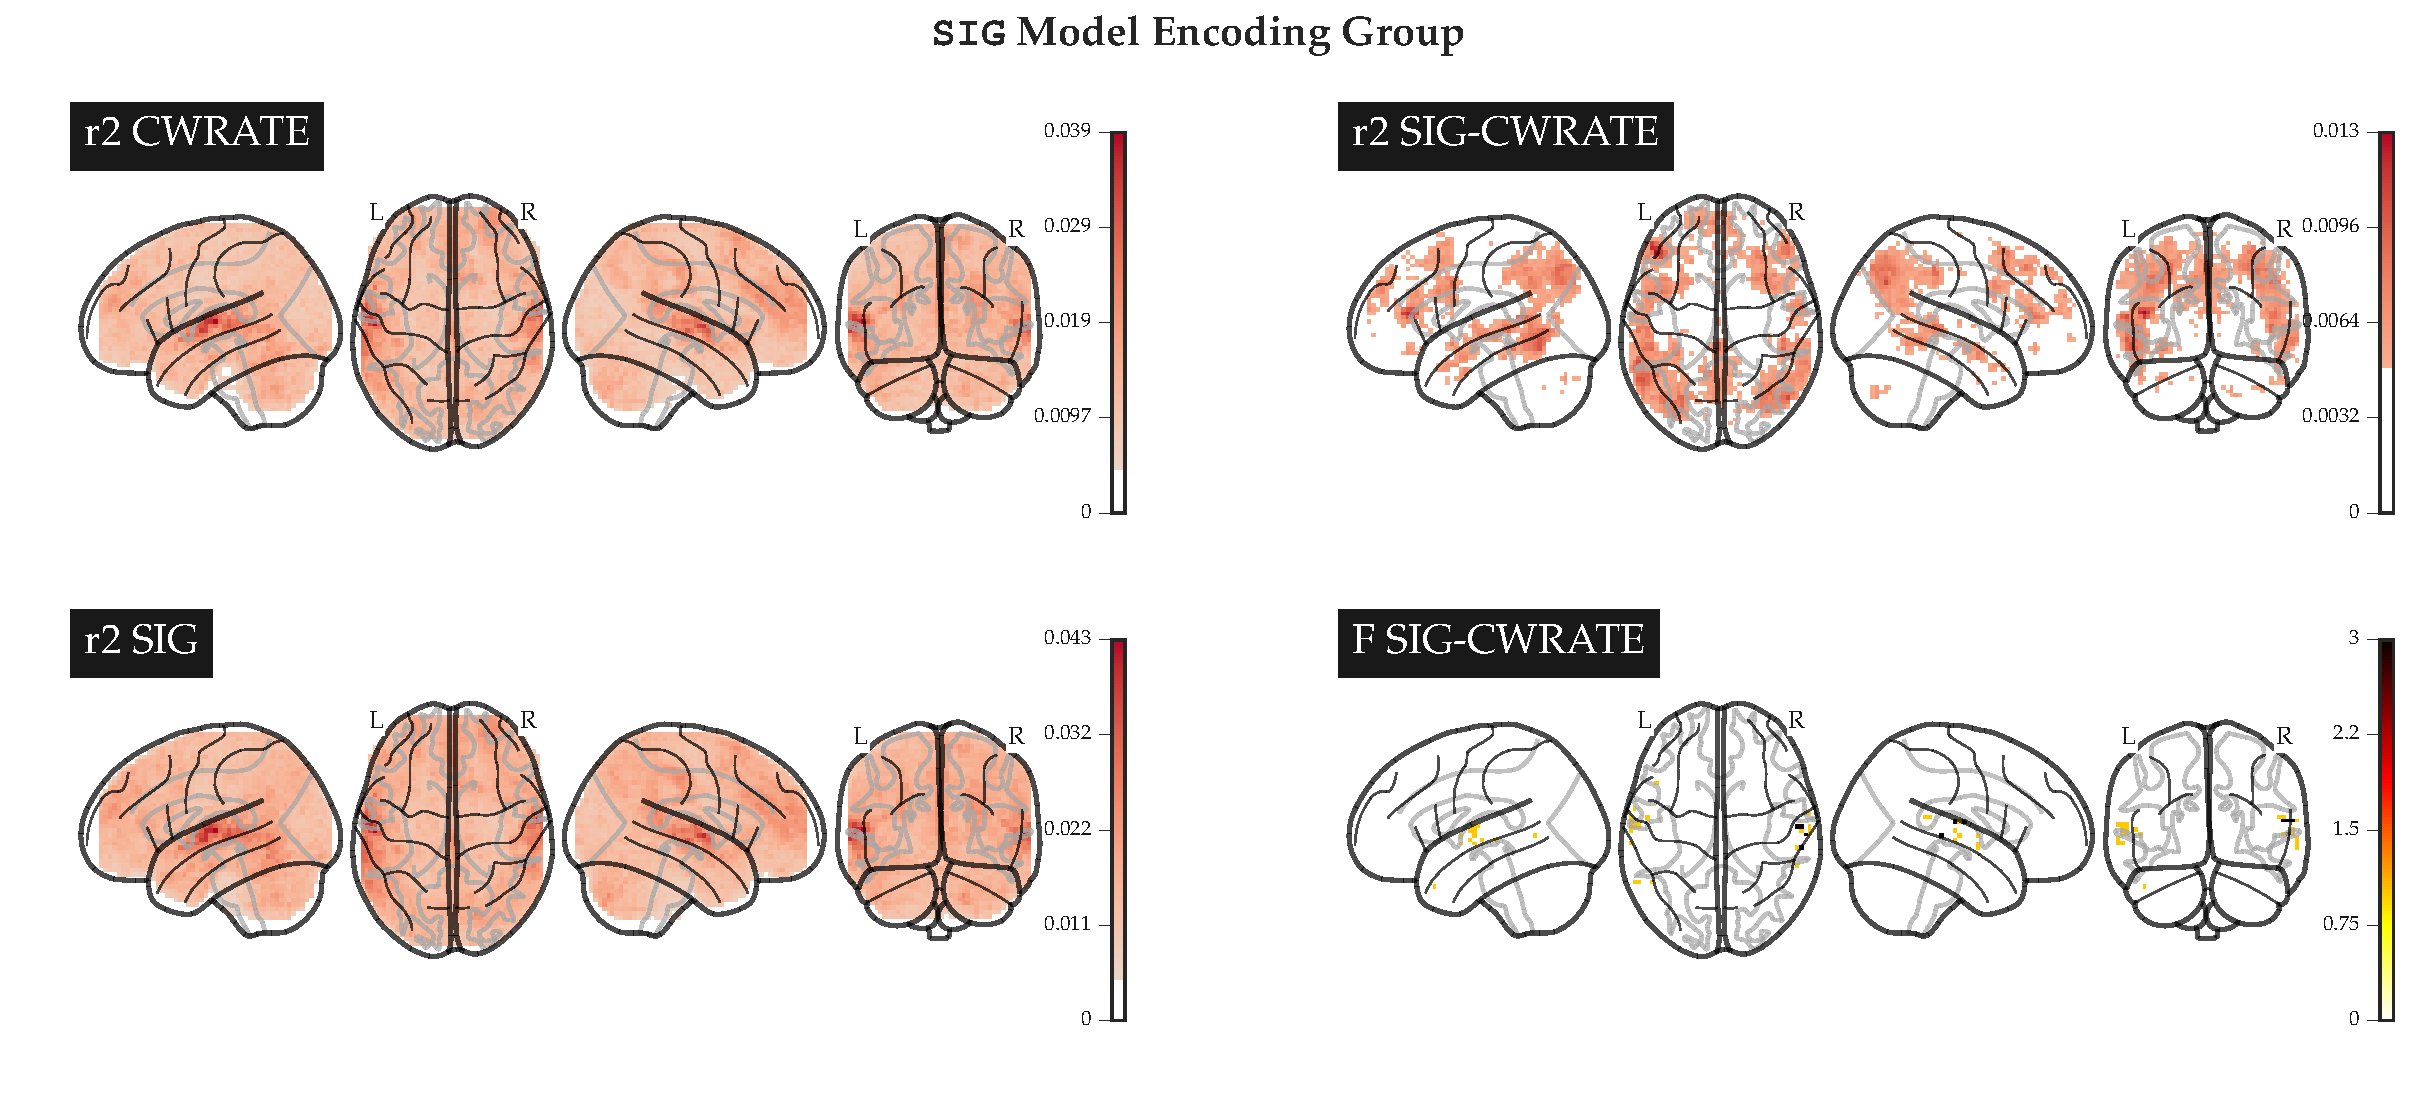
\includegraphics[width=.8\paperwidth]{Figures/SIG_ContrastMapG.pdf}
        }
        \caption[Encoding with \code{SIG} Features, Group]{\textbf{Right upper panel} shows that \code{SIG} better models left posteroinferior temporal gyrus (pITG), bilateral inferior frontal pars triangularis (IFGtri), SPL and AG. F-test in \textbf{right lower panel} reports significant voxels in right STG and trends in left STG (Table \ref{tab:Ftest}).} 
        \label{fig:SIG_ContrastMapG}
    \end{figure}
    
\code{SIG} contrast activates similar voxels as \code{SIM} except in the temporal region. \code{SIG} temporal improvements are found in posterior superior and inferior regions while \code{SIM} is more posterior middle (Figure \ref{fig:SIM_ContrastMapG} upper-right). The SPL position is located near the somatosensory cortex, and the angular cluster is more lateral and caudal. The coordinates are reported in Table \ref{tab:simImprovementClusters} (W=209, \(\Delta\)\code{r2}>0.0079, p-value<\(10^{-4.35}\) uncorrected).  Subject-wise results are available online\footnote{Whole-brain maps: \url{http://bit.ly/micipsa_sig_wholebrain}.}.

\subsection{\emph{Association} Nested Model}

\begin{figure}
    \centering
    \makebox[\linewidth]{
    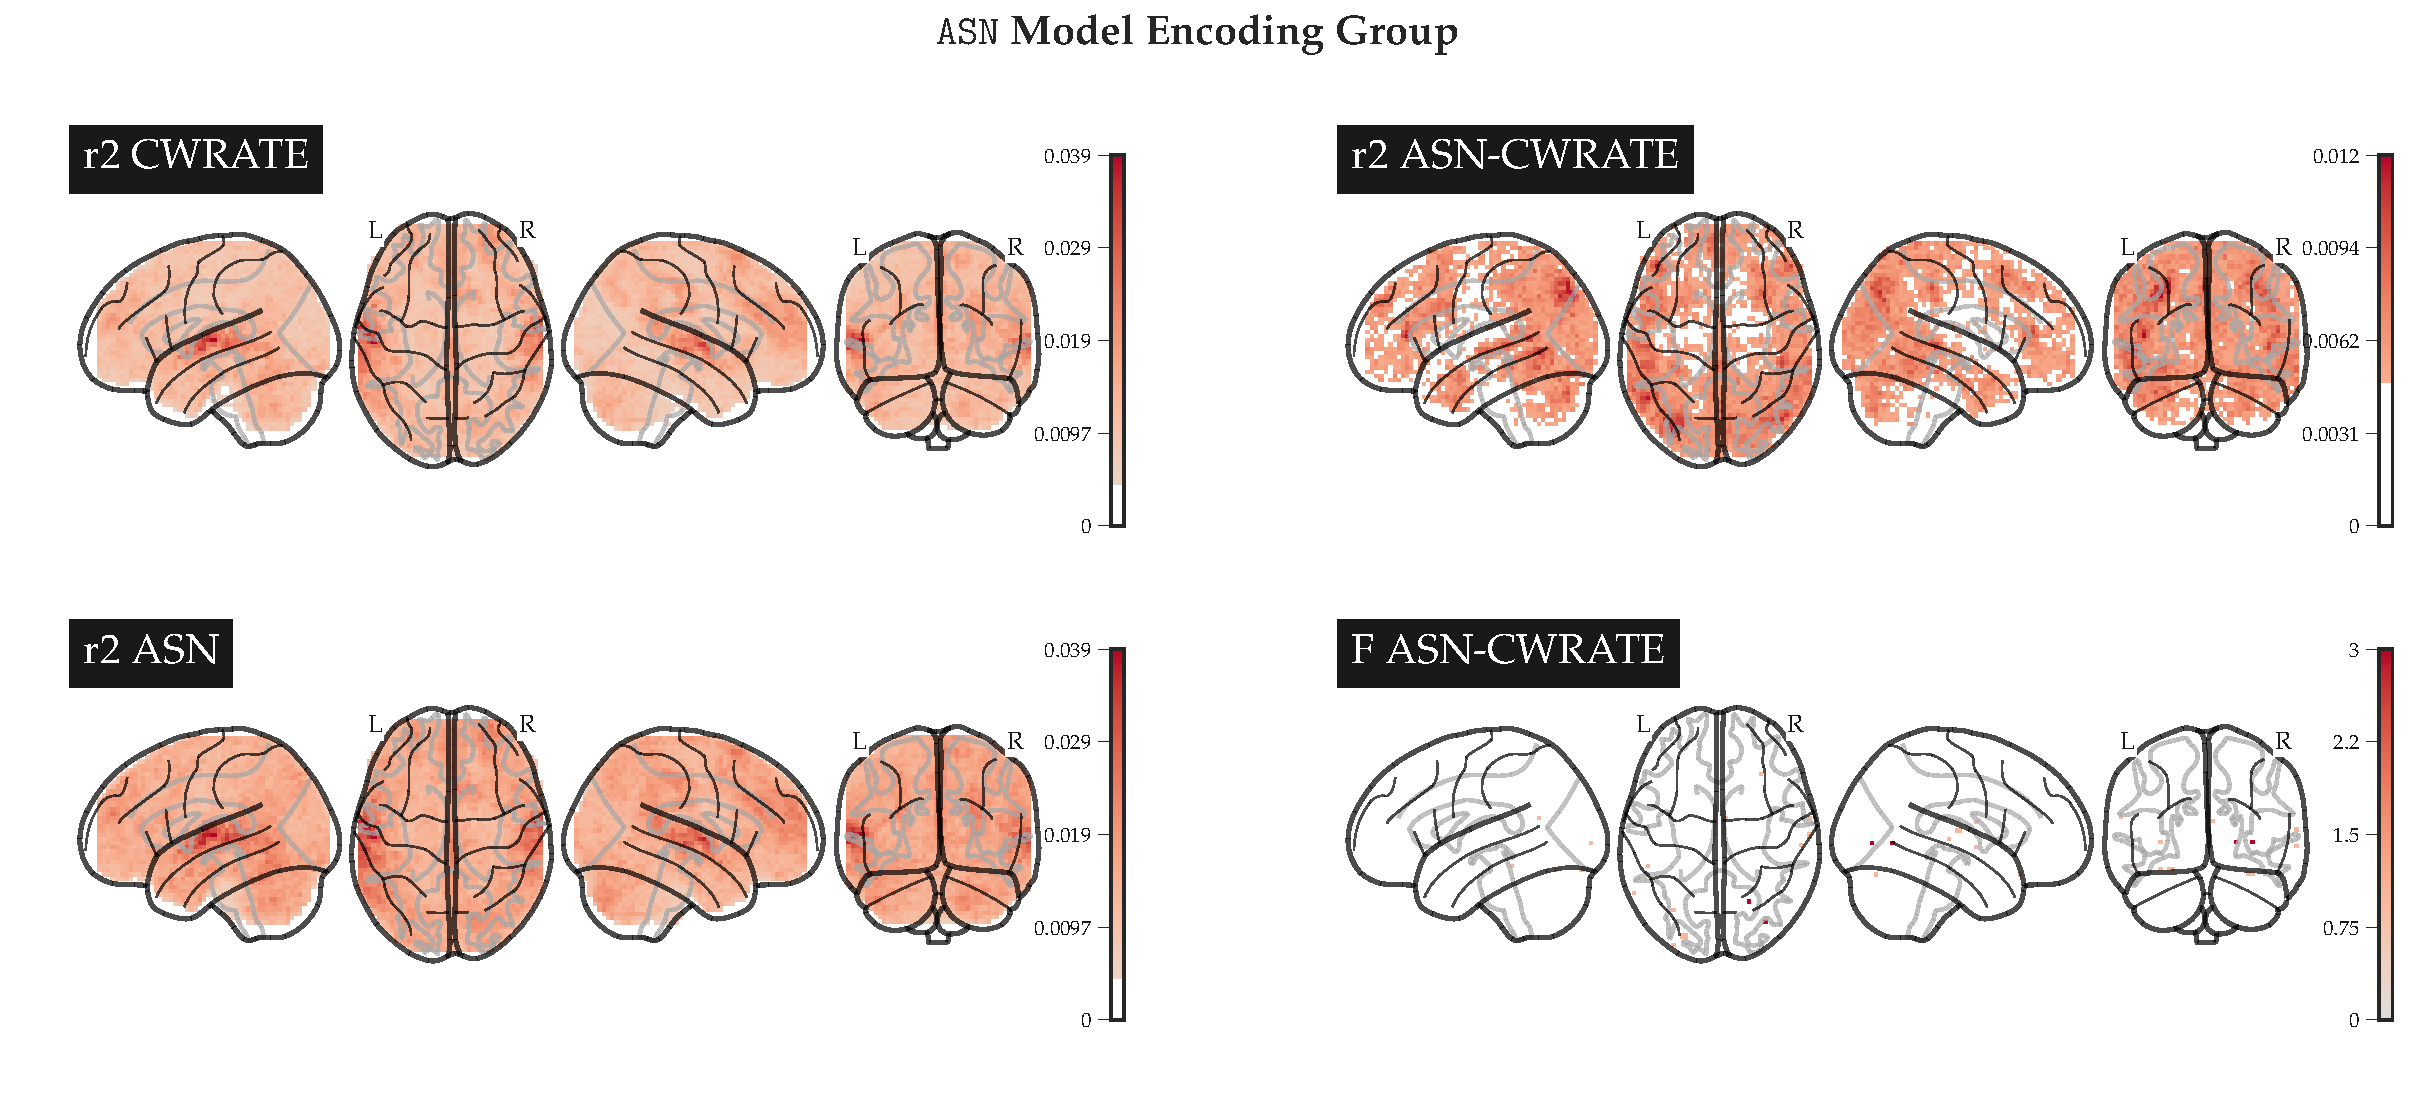
\includegraphics[width=.8\paperwidth]{Figures/ASN_ContrastMapG.pdf}
    }
    \caption[Encoding with \code{ASN} Features, Group]{Improvements of voxel-models are distributed in an extensive part of all lobes (\textbf{right upper panel}). The most improved voxels are located in bilateral MTG, IFGtri, left mid occipital gryus, right angular gyrus, left superior medial PFC, mid frontal cortex, mid cingulum (Table \ref{tab:asnImprovementClusters}). F-test in \textbf{right lower panel} reports significant voxels in right lingual BA19 and mid occipital area BA18 (Table \ref{tab:Ftest}).} 
    \label{fig:ASN_ContrastMapG}
\end{figure}

On adding \code{ASN} features on \code{BASE} features, the bilateral auditive cortices dominance is consistently kept (Figure \ref{fig:ASN_ContrastMapG}, Table \ref{tab:rmsCluters}). \code{ASN} brings voxel-model performance boost in an extensive cortical regions including left pFG, bilateral IFGtri, left MOG/BA39, right AG, left superior mPFC, mid frontal cortex, mid cingulate cortex (Table \ref{tab:asnImprovementClusters}, W=190, \(\Delta\)\code{r2}>0.0065, p-value<\(10^{-4.18}\) uncorrected). F-test results shows that \code{ASN} significantly improves isolated voxels (Table \ref{tab:Ftest}, p-value<0.05 voxel-wise multi-comparison corrected) in right lingual gyrus BA19 and BA18 (visual association). All reported regions are either associated to vision, or visual association, suggesting the modality-specificity of \association is consistent with the \code{ASN} construction.
Subject-wise results are available online\footnote{Whole-brain map: \url{http://bit.ly/micipsa_asn_wholebrain}.}.

 % right BA21 MTG [Senkowski, D., Schneider, T. R., Foxe, J. J., and Engel, A. K. (2008)., multisensory capabilities] Fusiform [within category Trafton, A. "How does our brain know what is a face and what’s not?" MIT News]



\subsection{\emph{Similarity}/\emph{Association} Contrast}

\subsubsection{\code{ASN} With \code{SIM}}

\begin{figure}
    \centering
    % \begin{minipage}[t]{\textwidth}
    \makebox[\linewidth]{
    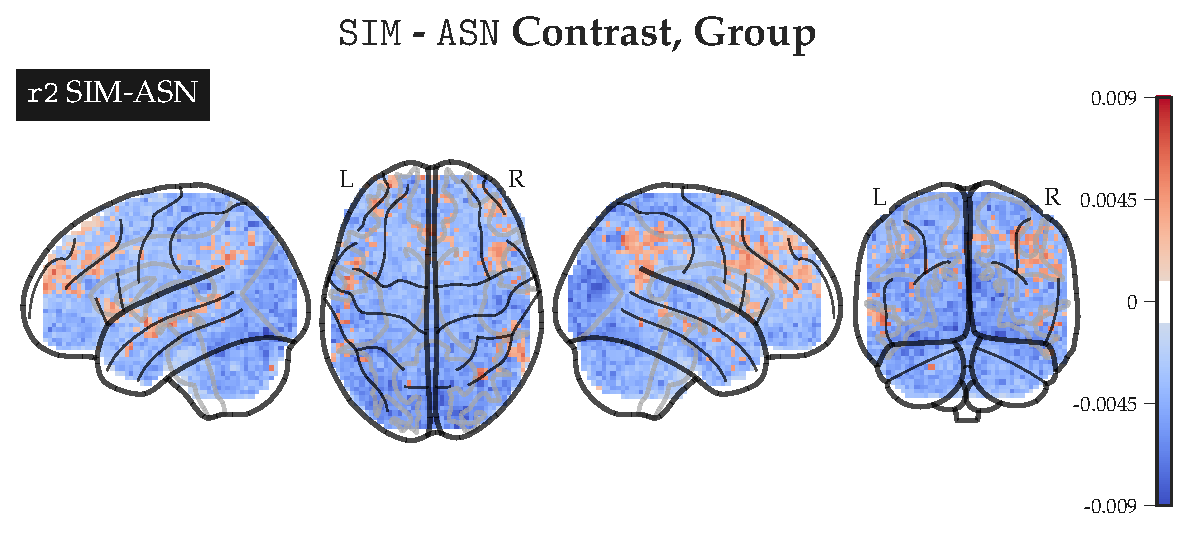
\includegraphics[width=.4\paperwidth]{Figures/EMB_SIM_ASN_r2_ContrastMapG.pdf}
    % % 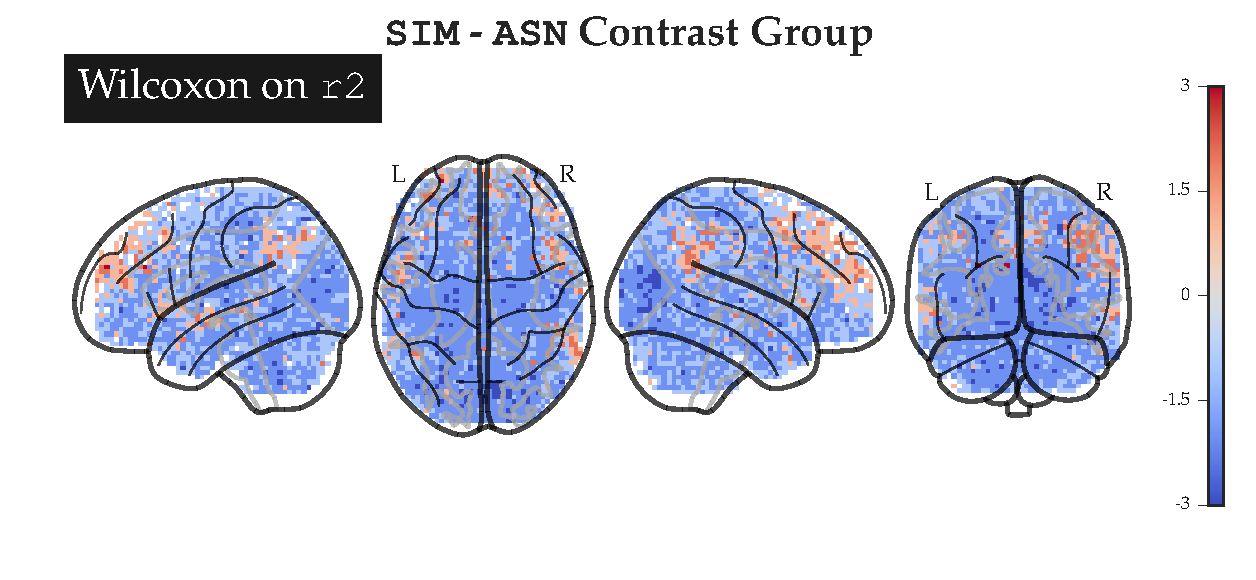
\includegraphics[width=.4\paperwidth, clip, trim=0cm,0cm,0cm, 1cm]{Figures/EMB_SIM_ASN_ContrastMapG.pdf}
    }
    % \end{minipage}
    % \begin{minipage}[t]{\textwidth}
    \makebox[\linewidth]{
        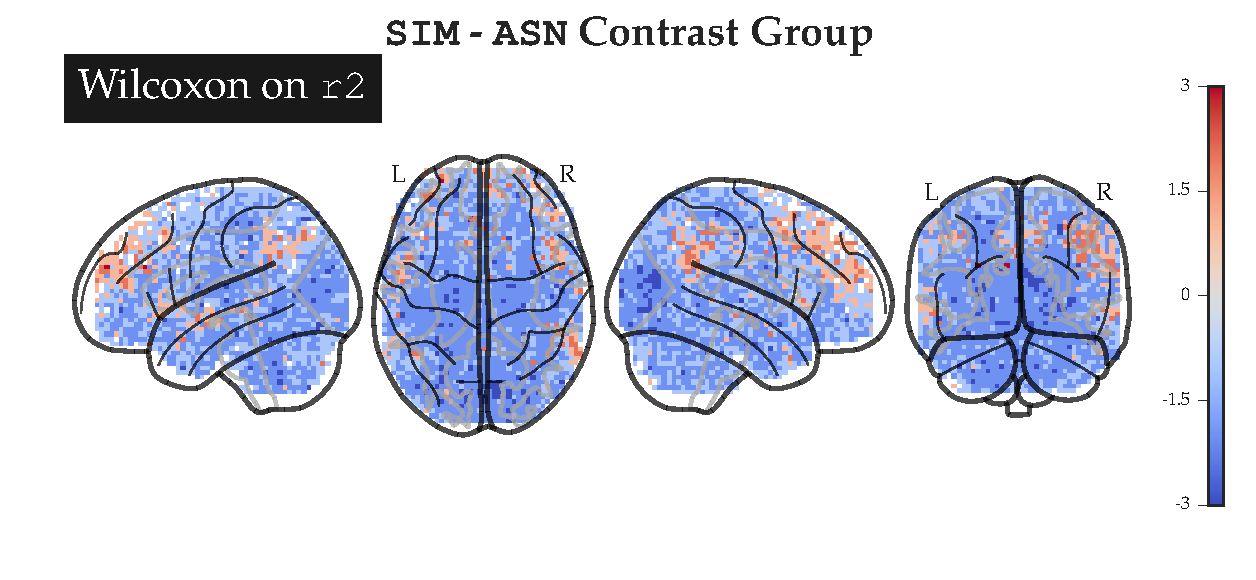
\includegraphics[clip, trim=0cm 0cm 0cm 1cm, width=.4\paperwidth]{Figures/EMB_SIM_ASN_ContrastMapG.pdf}
    }
    % \end{minipage}
    \caption[\code{SIM}-\code{ASN} Contrast, Group]{The differences of best voxel-model \code{r2}s are plotted in \textbf{upper panel}, significance levels in \textbf{lower panel}.} 
    \label{fig:EMB_SIM_ASN_ContrastMapG}
\end{figure}

Following the non-nested model comparison procedure, Section \ref{appsubsec:nonnestedcompres} suggests that first feature dimensions of \code{SIM} design matrices can be partially recovered by \code{ASN} model. Therefore, \code{ASN} might also be able to model voxels using less than 5 features from \code{SIM}, the result might thus underestimate \code{SIM} voxel extents and overestimate \code{ASN} ones. As the first 4 dimensions of \code{SIM} encodes primarily POS information (Section \ref{appsubsec:projectorvisu}), we performed ad-hoc regressions on \code{SIM} space but uses only lemmas from a certain grammatical category to rule out this confound (upcoming). 

Multiple indications on \code{ASN}'s richer semantic information including the explained variance ratio analysis (Figure \ref{fig:FreDecorVarRatio}) and the design matrix correlation analysis are consistent with the regression results: \code{ASN} scores are higher than \code{SIM} in average (Figure \ref{fig:SIM_ASN_Distribution} right), most of cortical areas respond better to \code{ASN} models (Figure \ref{fig:EMB_SIM_ASN_ContrastMapG}). Only two small significant clusters are found for \code{SIM} in left superior frontal cortex BA10 and left anterior cingulum cortex (ACC) (Table \ref{tab:simasnContrastClusters_sim}, W>6945, \(\Delta\)\code{r2}>0.0068, p-value<0.05 voxel-wise multi-comparison corrected). BA10 is suggested to be linked to memory recall and executive functions, and ACC BA32 to error detection and social evaluation. Left aSTG, right pSTG, right pSTS BA22 and left aSTS/mid TP are also reported (p<0.001 uncorrected). 

\code{ASN} found 17 small culsters \code{ASN} (Table \ref{tab:simasnContrastClusters_asn}) in bilateral visual association areas (BA18), primary visual areas (BA17), ventrotemporal areas (ventroinferior ITG, parahippocampal gyrus), left SPL, left thalamus and bilateral cerebellum. The temporal locations are linked to social interactions and sarcasm (parahippocampal) \parencite{rankinDetectingSarcasmParalinguistic2009}. No prior evidence implicates \similarity involvement for other found sites. Subject-wise results are available online\footnote{Whole-brain maps: \url{http://bit.ly/micipsa_sim_asn_contrast}.}.

The reported clusters for \code{SIM} are composed of 4 to 5 voxels. In our ROI analysis, ROIs larger than 26 voxels are used, thus none of the ROI revealed significance for \code{SIM}. As \code{ASN} has an overall dominance for almost all brain regions, small ROIs located in left middle/posterior STG and large anatomical structures including IPL and TL all revealed their preference for \code{ASN} model. 

\begin{figure}
    \centering
    \makebox[\linewidth]{
    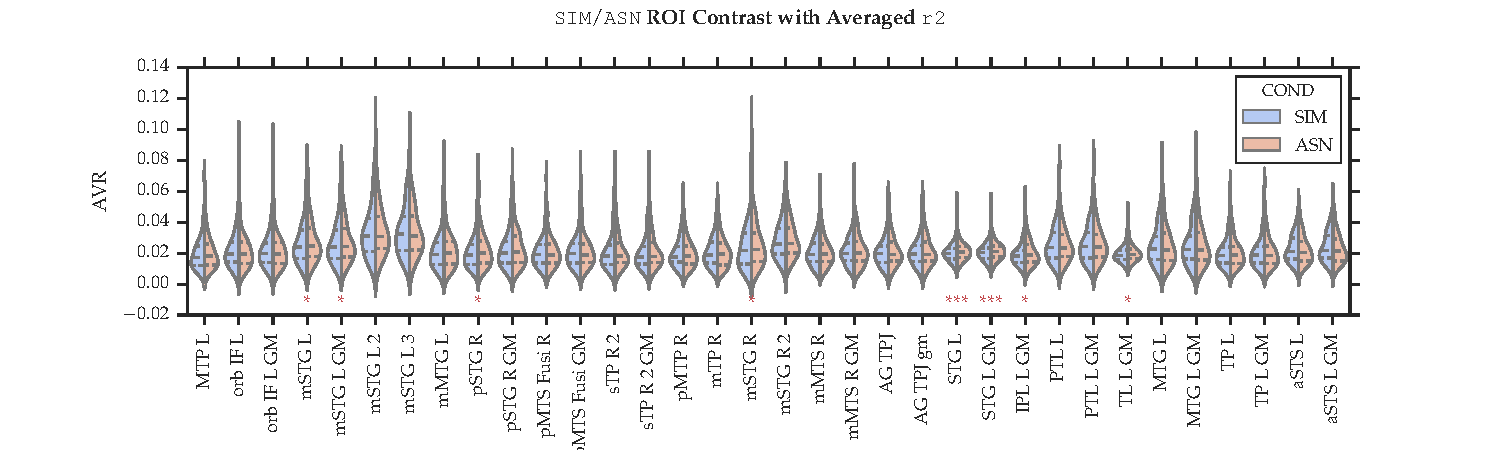
\includegraphics[width=\paperwidth]{Figures/SIM_ASN_ROI.pdf}
    }
    \caption[\code{SIM}-\code{ASN} ROI Contrast, Group]{*: p<0.05 uncorrected, ***: 0.05 ROI-wise multi-comparison corrected. Red color for \code{ASN}.\\ The average \code{r2} of voxels in a ROI is computed. We select only ROIs with scores>0.02 in either of \code{SIM} and \code{ASN} models. ROIs are of minimum size of 26 voxels (radius of 7 mm). None of the tested ROI reveals a significant mean difference in preference for \code{SIM}. ROIs in left middle-posterior STG, left inferior parietal lobe and left temporal lobe respond better to \code{ASN} model.} 
    \label{fig:SIM_ASN_ROI}
\end{figure}


\subsubsection{With \code{SIG}}

In general \code{SIG} outperforms \code{SIM}. The model performance contrast indicates a preference for \code{SIG} over \code{ASN} in right angular and precuneus (Figure \ref{fig:EMB_SIG_ASN_ContrastMapG}, Table \ref{tab:sigasnContrastClusters_sig}, \(\Delta\)\code{r2}>0.0073, p-value<0.05 voxel-wise multi-comparison corrected). Temporal sites including bilateral pSTG (PA, BA41) and left aSTG are also reported before correction. Only the left aSTG located in BA22 was recurrent with \code{SIM}-\code{ASN} contrast. The ROI analysis find \code{SIG} preference in bilateral mSTG before correction (Figure \ref{fig:SIG_ASN_ROI}).

Consistent with former contrast with \code{SIM}, \code{ASN} is activated for bilateral calcarine (BA18, 18) in primary and associational visual area. ROIs in left aMTG, left a/mFG, left TPS, right TPL, IFGober, IFGtri and bilateral aTL and TP are found significantly more correlated with \code{ASN} (Table \ref{tab:sigasnContrastClusters_asn}).

The evidences from two contrasts only shares one small left aSTG site. Other reported temporal areas' specificity in two semantic principles do not lead to a consistent conclusion.